\section{Results}
\label{results}

We test our implementation by simulating a rotating galaxy.
To this end, we place $N = \num{40000}$ particles at random positions inside a disk with radius \num{1.25} in the center of a square domain of size $50 \times 50$.
The positions are sampled uniformly in polar coordinates which results in a higher particle density in the center of the galaxy.
All particles have the mass $m = \nicefrac 1N$ and an initial velocity in tangential direction with magnitude $0.9 \sqrt{r}$, where $r$ is the distance of the particle to the center of the disk.
This results in a rotating disk of particles such that gravitational and centrifugal forces roughly balance each other.
Furthermore, we use the velocity-Verlet algorithm \cite{groot} with time steps of size $\mathrm{dt} = 0.01$, expansions with $P=5$ and store up to $s = \num{64}$ particles per leaf.
\cref{fig:res-galaxy} shows the distribution of the stars after different number of time steps.
We observe that patterns in the particle distribution evolve which eventually form the typical spiral arms.

\begin{figure}
  \centering
  \subfloat[0]{
    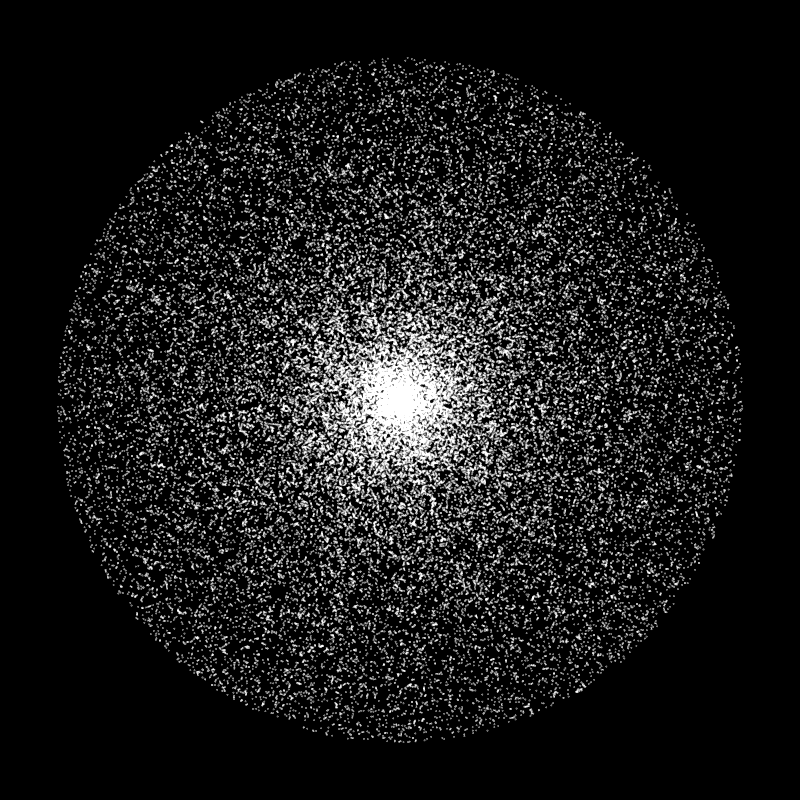
\includegraphics[width = 0.3 \textwidth]{img/galaxy-000.png}
  }
  \subfloat[1000]{
    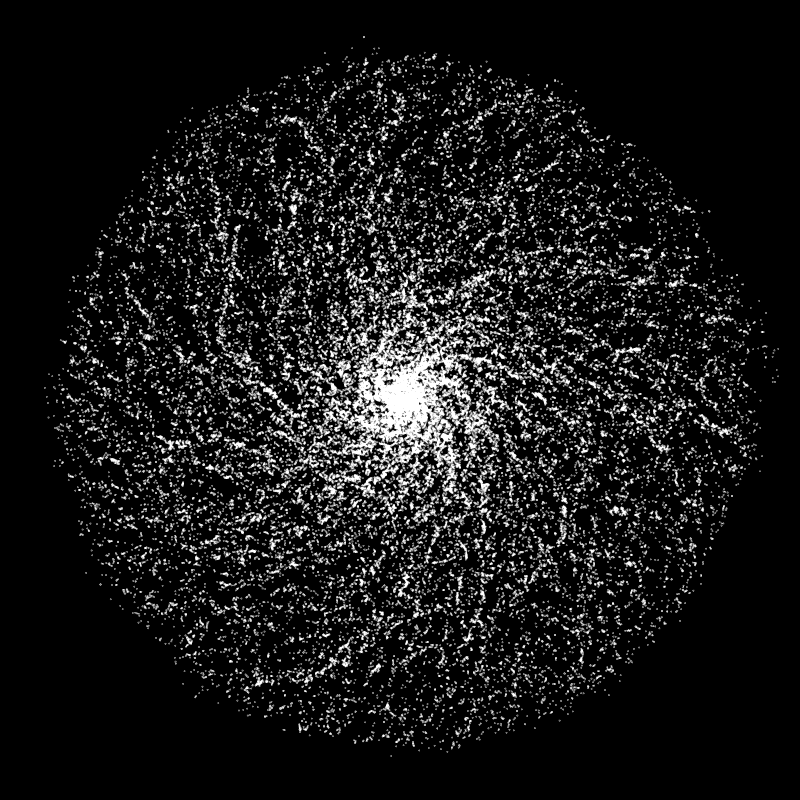
\includegraphics[width = 0.3 \textwidth]{img/galaxy-100.png}
  }
  \subfloat[2000]{
    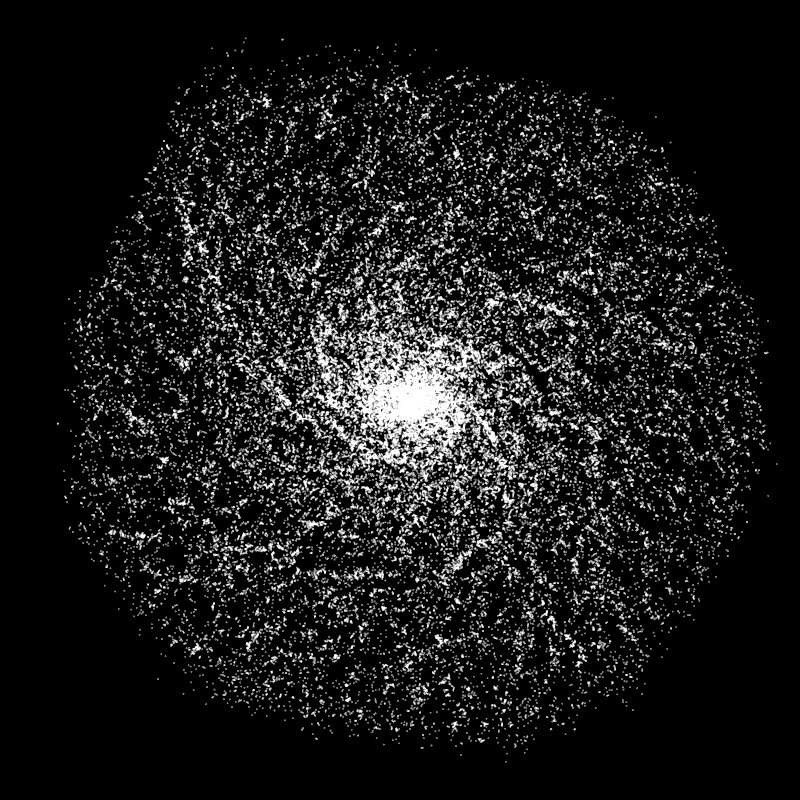
\includegraphics[width = 0.3 \textwidth]{img/galaxy-200.png}
  }

  \subfloat[3000]{
    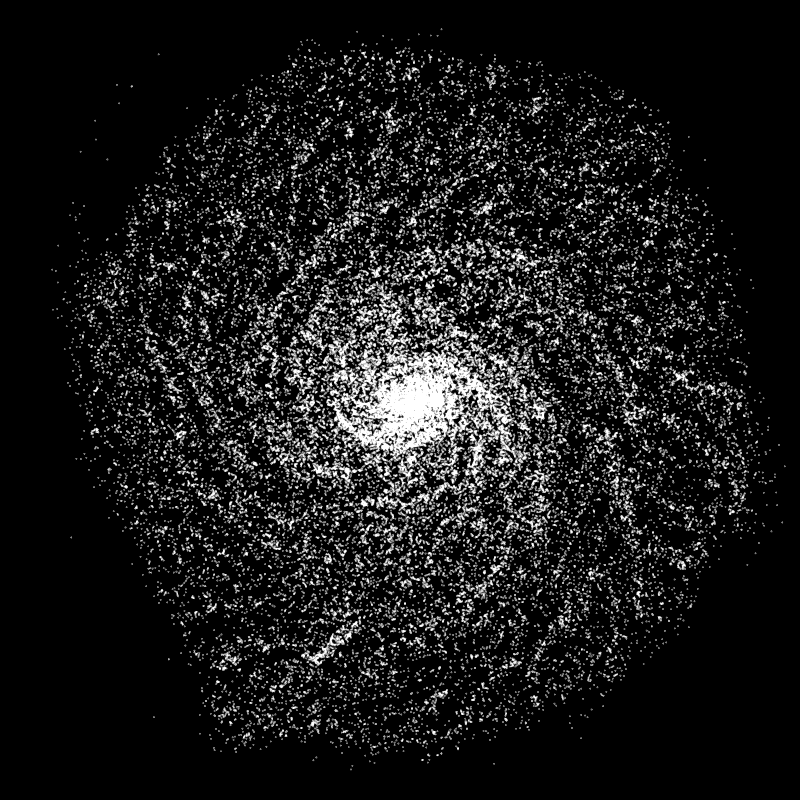
\includegraphics[width = 0.3 \textwidth]{img/galaxy-300.png}
  }
  \subfloat[4000]{
    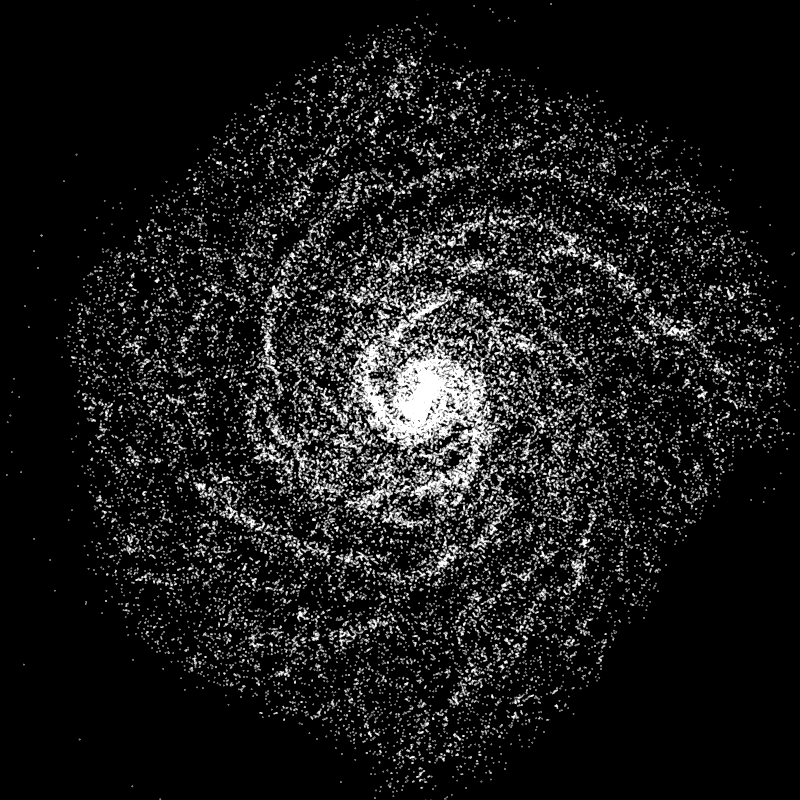
\includegraphics[width = 0.3 \textwidth]{img/galaxy-400.png}
  }
  \subfloat[5000]{
    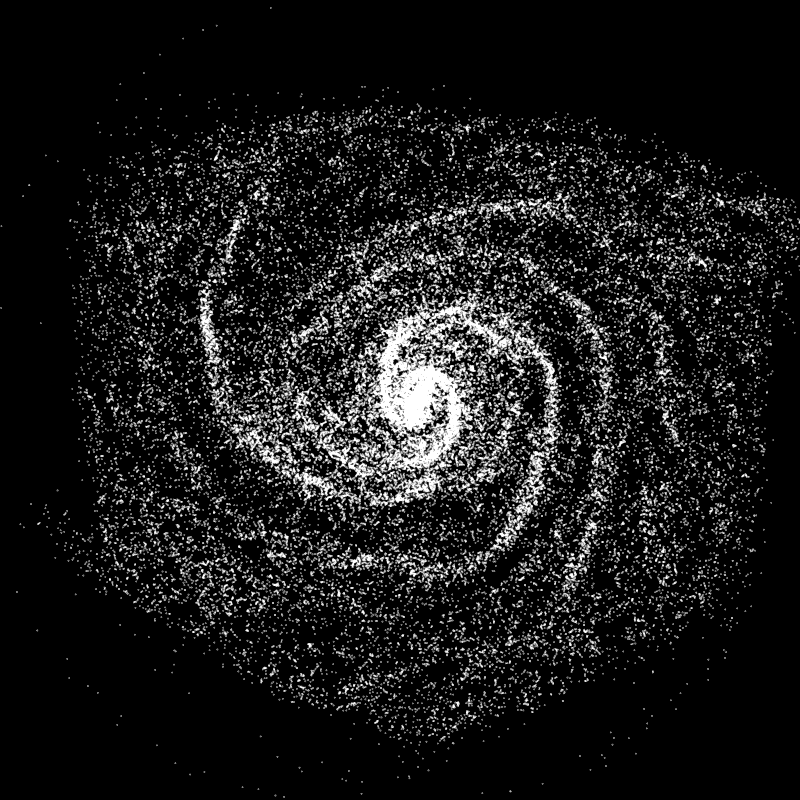
\includegraphics[width = 0.3 \textwidth]{img/galaxy-500.png}
  }
  \caption{Results of the galaxy simulation at different time steps.}
  \label{fig:res-galaxy}
\end{figure}

\begin{figure}
  \centering
  \subfloat[Scaling behavior with maximal 50 particles per leaf]{
    \label{fig:measure:n}
    \begin{tikzpicture}[scale=0.65]
      \begin{axis}[ xlabel = {Number of particles}
                  , ylabel = {Wall time [\si{s}]}
                  , xmode  = log
                  , ymode  = log
                  , width  = 0.7\textwidth
                  , height = 0.7\textwidth
                  , grid   = both
                  , grid style                    = {line width=.2pt, draw=gray!10}
                  , major grid style              = {line width=.2pt, draw=gray!50}
                  , legend pos                    = {north west}
                  , legend cell align             = {left}
                  , every axis plot/.append style = {ultra thick}
                  , cycle list name               = mark list
                  ]
        \addplot+[highlight] table [x=nParticles,y=time] {data/scaling_time-per-particles-leaf050-dt0.1-nSteps500.txt};
        \addlegendentry{Measurements};

        \addplot[ifi, domain=3e1:5e2] {x^2 * 2.45234e-6};
        \addplot[ifi, domain=5e2:1e6] {x   * 0.00122617};
        \fill[ifi] (500, 0.613085) circle (2pt);
        \addlegendentry{$\mathcal{O}(N^2)$ and $\mathcal{O}(N)$ for comparison};
      \end{axis}
    \end{tikzpicture}
  } \subfloat[Runtime for varying number of particles per leaf with $N = 2^{12}$]{
    \label{fig:measure:s}
    \begin{tikzpicture}[scale=0.65]
      \begin{axis}[ xlabel = {Maximum number of particles per leaf}
                  , ylabel = {Wall time [\si{s}]}
                  , width  = 0.7\textwidth
                  , height = 0.7\textwidth
                  , grid   = both
                  , grid style                    = {line width=.2pt, draw=gray!10}
                  , major grid style              = {line width=.2pt, draw=gray!50}
                  , minor x tick num              = 1
                  , minor y tick num              = 1
                  , every axis plot/.append style = {ultra thick}
                  , cycle list name               = mark list
                  ]
        \addplot+[highlight] table [x=s,y=time] {data/time-per-s-n04e3-dt0.1-nSteps500.txt};
      \end{axis}
    \end{tikzpicture}
  }
  \caption{Measured runtime with varying number of particles and maximum particles per leaf node}
\end{figure}

In \cref{fig:measure:n} you can see the scaling behavior of the \gls{fmm} for our galaxy example with maximal 50 particles per leaf node.
For easier interpretation we also show how quadratic and linear scaling would look like.
For small number of particles ($N < 500$) the algorithm scales approximately quadratically.
This is to be expected since all particles could fit into ten leaves which means that almost all interactions are calculated directly.
On the other hand, we see that the complexity approaches $\mathcal{O}(N)$ for larger $N$.

Furthermore, we investigate the effect that the maximum number $s$ of particles per leaf has on the runtime.
\cref{fig:measure:s} collects benchmark results for $N = 2^{12} = 4096$.
We observe the shortest runtimes with values of $s$ between 25 and 64.
The optimum among the tested values is $s=50$, which reduces the runtime by a factor of six compared to $s=1$.
